\documentclass{llncs}
%\documentclass[a4paper,10pt]{article}
%\usepackage{amsmath}
\usepackage{amsfonts}
\usepackage[blocks]{authblk}
\usepackage[utf8x]{inputenc}
\usepackage{graphicx}
\usepackage[caption=false,font=footnotesize]{subfig}
\usepackage{url}
\usepackage{array}
\usepackage{rotating}
\usepackage{wasysym}
\usepackage{multirow}
\usepackage{color}
\usepackage{calc}
\usepackage{listings}

\pdfminorversion=5

\newcommand{\ta}{Timed Automaton}
\newcommand{\tas}{Timed Automata}
\newcommand{\nat}{\mathbb{N}}
\setlength{\belowcaptionskip}{-10pt}


\title{Towards interactive model checking\\of biological pathway dynamics}

\author{Stefano Schivo${}^\star$
\and Jetse Scholma${}^\star$
\and Paul E. van der Vet
\and Marcel Karperien
\and Janine N. Post
\and Jaco van de Pol${}^{\star \star}$
\and Rom Langerak${}^{\star \star}$}

\institute{University of Twente, Enschede, The Netherlands}



\date{}
\pagestyle{plain}

\begin{document}

\maketitle
%\thispagestyle{empty}

\let\oldthefootnote\thefootnote
\renewcommand{\thefootnote}{\fnsymbol{footnote}}
\footnotetext[1]{These authors contributed equally to this work.}
\footnotetext[2]{Corresponding authors.}
\let\thefootnote\oldthefootnote



\begin{abstract}

Biological systems such as regulatory or gene networks can be
seen as a particular type of distributed systems, and for this reason
they can be modeled with the same tools that were developed in the
computer science context. However, tools designed to model distributed
systems often require a computer science background, making their use
less attractive for biologists. ANIMO (Analysis of Networks with
Interactive MOdeling) was built with the aim to provide biologists
with access to the powerful modeling formalism of Timed Automata
in a user friendly way. Continuous dynamics is handled by discrete approximations.

This brings computational support closer to the biological laboratories, 
where large amounts of data are generated on a daily basis. Thanks to 
computational models, biological data can be analyzed in different ways, 
helping biologists to formulate new hypotheses, drive experimental research 
and share knowledge on biological processes.

In this paper we introduce an improved modeling approach that allows us
to considerably increase ANIMO's performances, opening the way for the
analysis of bigger models. Moreover, this improvement makes the introduction
of model checking in ANIMO a realistic feature, allowing for
reduced computation times. The user interface of ANIMO allows to rapidly
build non-trivial models and check them against properties formulated in
a human-readable language, making modeling a powerful
support for biological research.

\end{abstract}

\section{Introduction}\label{sec:introduction}

To study the possible causes of a disease and design effective cures it is 
necessary to closely study the behavior exhibited by biological cells under particular conditions.
A \emph{signaling pathway} describes the chain of interactions occurring
between the reception of a \emph{signal} and the response with which the cell
reacts to such signal. 
A signal is typically represented by a substance which can bind
to specific receptors on the cell surface, activating them.
\emph{Active} molecules relay the signal inside the cell by activating
other molecules until a target is reached. The target of a signaling pathway is usually a transcription
factor, a molecule with the task of controlling the production of some protein. Such regulation is considered to be the response of the cell to the received signal.
% Experimental evidence has shown that the interactions leading to a cellular response assume
% more often the shape of a network than that of a simple chain of signal relays.

The current knowledge on signaling pathways (mostly organized in databases such as KEGG~\cite{kegg}
or PhosphoSite~\cite{phosphosite}) suggests that the interactions involved in a cellular response assume more often
the shape of a network than that of a simple chain of signal relays.
Such networks are typically highly connected, involving feedback loops and crosstalk
between multiple pathways, making it difficult for the human
brain to grasp their dynamic behavior.
For this reason, a computational support is required when studying non-trivial biological networks.

A number of software tools are available
for modeling complex networks of biochemical interactions~\cite{bio-pepa,blenx,copasi,e-cell,gna}.
These tools significantly contribute to the process of formalizing the knowledge on biological
processes, rendering them amenable to computational analysis.
However, a lack of familiarity with the formalisms underlying many available tools
hampers their direct application by biology experts.
ANIMO (Analysis of Networks with Interactive MOdeling,~\cite{animo-site,animo-ieee,animo-gene}) is a software tool
based on the formalism of \tas~\cite{timed-automata-alur} that supports the
modeling of biological signaling pathways
by adding a dynamic component to traditional static representations of signaling networks.
ANIMO allows to compare the behavior of
a model with wet-lab data, and to explore such behavior in a user-friendly way.
In order to achieve a good level of user-friendliness for a public of biologists, the complexity of \tas\ is hidden \emph{under the hood},
presenting ANIMO as an app for Cytoscape~\cite{cytoscape}, a tool specifically developed for visualizing 
and elaborating biological networks. Signaling networks are represented in ANIMO using
the nodes-edges notation normally used in the context of biology (see Fig.~\ref{fig:small-example-net}).

Previously, ANIMO supported only interactive exploration of network dynamics based on simulation runs. 
Model checking queries could be answered through the UPPAAL tool~\cite{uppaal}, but
the required knowledge of temporal logic together with the usually long response times slowed down the investigation process.
In order to encourage the use of model checking on non-trivial models of
signaling networks, we updated ANIMO with a new \tas\ model (presented here). This marks a relevant improvement in terms of
performances with respect to the model previously used in ANIMO. Moreover, consistently with the intents of our tool, we
implemented also a user interface for the definition of model checking queries in ANIMO. This allows a
user to interrogate an ANIMO model without requiring previous experience in temporal logics. These new
features are available in the latest version of ANIMO, which was recently reimplemented as a Cytoscape 3 app~\cite{animo-app-site}:
this lets users profit of the additional analysis features made available by the other apps in the Cytoscape environment.

% The rest of the paper is organized as follows:
% Section~\ref{sec:basics} introduces the basic aspects
% of signaling pathways, \tas\ and ANIMO; Section~\ref{sec:animo-new} illustrates a new way of using \tas\ to model
% activity-based networks;
% Section~\ref{sec:animo-comparison} shows a comparison between the new modeling approach and the
% one previously used in ANIMO,
% focusing on model analysis performances; Section~\ref{sec:animo-model-checking-ui} describes the
% interface additions to make model checking accessible to ANIMO users;
% Section~\ref{sec:conclusion} concludes the paper, discussing future work.
The paper continues as follows.
After introducing the basic concepts in Section~\ref{sec:basics}, we illustrate in
Section~\ref{sec:animo-new} a new way of using \tas\ in ANIMO.
In Section~\ref{sec:animo-comparison} we present a comparison between the new modeling approach and the
one previously used in ANIMO,
focusing on model analysis performances. In Section~\ref{sec:animo-model-checking-ui} we describe
how model checking was made accessible to ANIMO users.
We conclude the paper with Section~\ref{sec:conclusion}, discussing future work.

\section{Preliminaries}\label{sec:basics}

\subsection{Signaling pathways in biology}\label{sec:biologia}
A signaling pathway is an abstract representation of the reactions occurring inside a biological cell when, e.g., a
signaling substance comes in contact with the cell surface receptors.
In this setting, a reaction is the interaction between
two components: the upstream enzyme (the molecule holding the active role in the reaction) and the downstream
substrate (the passive molecule). The enzyme can be for example a kinase, which attaches a phosphate group to its
substrate, performing a phosphorylation: this determines a change in the shape of the substrate
and consequently a new function (Fig.~\ref{fig:small-example-biology}).
The new state reached by the substrate
is often called \emph{active}: if the substrate of the reaction is itself a kinase, it can then proceed in passing
on the signal by activating its own target molecule, continuing a chain of reactions leading to the target
of the signaling chain. Such target is usually a transcription factor, i.e. a molecule that influences
the genetic response of the cell, for example promoting the production of a particular protein.

Pathways are traditionally represented in a nodes-edges form (see Fig.~\ref{fig:small-example-net}),
with nodes representing molecular species and arcs standing for reactions, where $\rightarrow$ represents
activation and $\dashv$ represents inhibition (i.e. inactivation). 

\def\scalaRete{0.16}

\begin{figure}[htbp]
\centering
\subfloat[\label{fig:small-example-net}]{
\includegraphics[scale=\scalaRete]{images/tkk_tk_t_tutto_networkOnly}} \qquad \qquad
\subfloat[\label{fig:small-example01}]{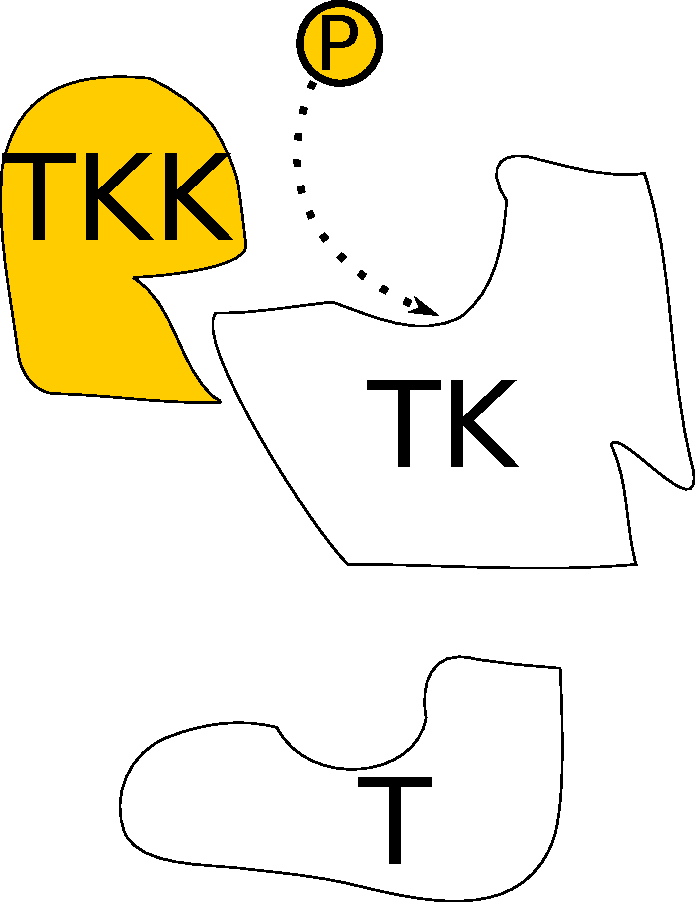
\includegraphics[scale=\scalaRete]{images/tkk_tk_t_tutto01}} \qquad \qquad
\subfloat[\label{fig:small-example02}]{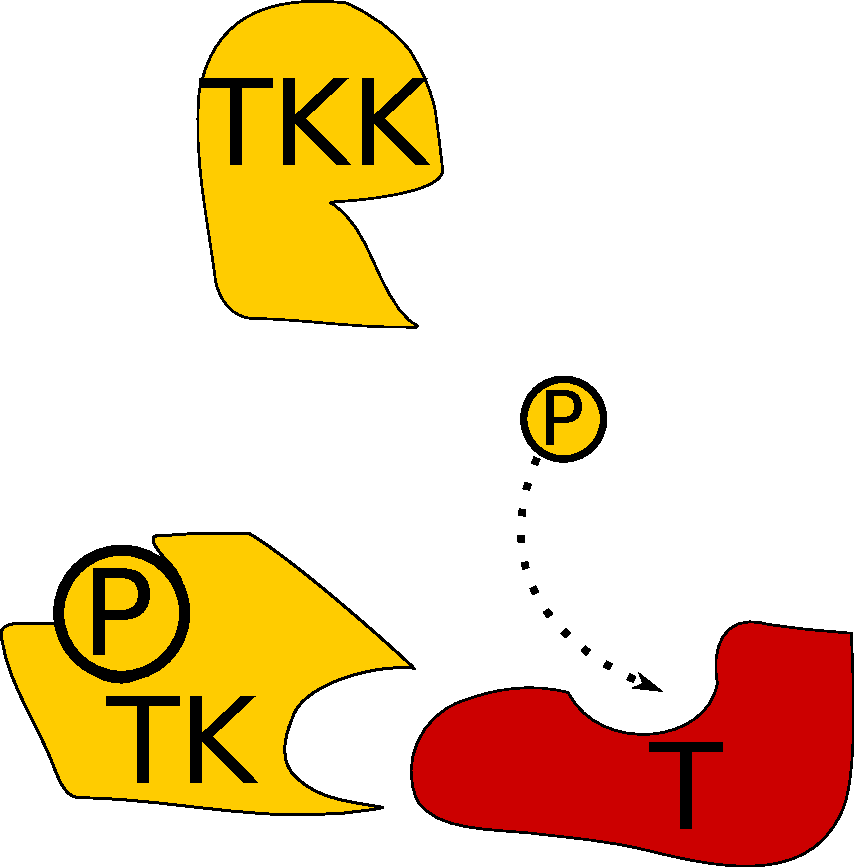
\includegraphics[scale=\scalaRete]{images/tkk_tk_t_tutto02}} \qquad \qquad
\subfloat[\label{fig:small-example03}]{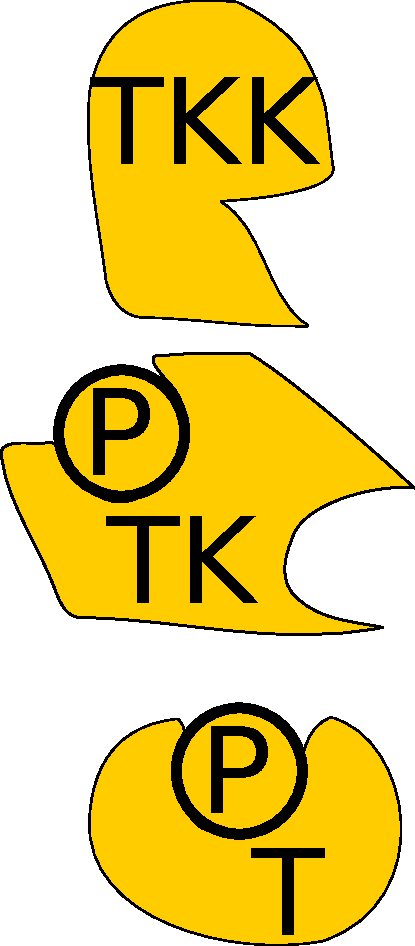
\includegraphics[scale=\scalaRete]{images/tkk_tk_t_tutto03}}
\caption{A kinase signaling network represented in the nodes-edges form {\bf\protect\subref{fig:small-example-net}}
and its evolution represented by abstract molecular interactions
({\bf\protect\subref*{fig:small-example01}\--{}\protect\subref*{fig:small-example03}}).
{\sf T} is the target of the signaling pathway, {\sf TK}
is the kinase that activates {\sf T}, and {\sf TKK} is the kinase that activates {\sf TK}.
{\bf\protect\subref{fig:small-example01}} An already active (yellow) {\sf TKK} can bind to
an inactive (empty) {\sf TK}, catalyzing its phosphorylation (i.e. binding of a phosphate group, {\sf P}).
This causes a change in the shape of {\sf TK}, activating its enzymatic function {\bf\protect\subref{fig:small-example02}}.
The active {\sf TK} can in turn activate its target {\sf T}, enabling it to carry out its function {\bf\protect\subref{fig:small-example03}}.
% {\bf\protect\subref*{fig:small-example-net}} represents the initial state of the network in the
% traditional nodes-edges form.
}\label{fig:small-example-biology}
\end{figure}

% \setlength{\abovecaptionskip}{2pt}

The current knowledge on signaling pathways~\cite{kegg,phosphosite} evidences the fact
that signaling interactions are rarely a simple chain of activations as represented in Figure~\ref{fig:small-example-net}.
More often, they assume the shape of a network with multiple feedback loops and crosstalk from different signaling sources.
This complexity is an added difficulty for the study of such networks, reducing the possibilities
%for the human brain alone
to deduce the dynamic behavior of a signaling network by inspecting its static representation.
For this reason, an efficient computational support is essential when representing and analyzing the behavior
of complex signaling networks.


\subsection{\tas}\label{sec:TA}
\renewcommand{\ta}{TA}
\renewcommand{\tas}{TA}
Timed Automata (\tas) are finite-state automata enriched with real-valued clocks
and synchronization channels. All clocks in a \tas\ system advance with the same rate,
and transitions between the locations of an automaton
depend on conditions on clocks. In particular, a \emph{guard} defines when a transition
may be taken, while an \emph{invariant} is the condition for permanence in a location.
A transition can also allow two automata to \emph{synchronize},
with each participant performing one of two complementary actions (\emph{input} and \emph{output})
on a synchronization channel. A set of clocks may also be reset by a transition, causing them to restart from 0.

The models we will present here were implemented using the software tool UPPAAL~\cite{uppaal}, which adds a number of features
to the basic definition of \tas. Some of these extensions include: support for integer variables in addition to clocks,
broadcast synchronization channels (one sender, many receivers), definition of C-like functions to perform more 
operations besides clock resets.
UPPAAL also allows for a special type of locations, named \emph{committed} (marked with a {\sf C} in the graphical representation).
As long as an automaton is in a committed location, time is not allowed to flow. This feature can be used for example to perform immediate
updates to local variables before letting the computation proceed. Examples of the listed features are found in the
\tas\ model in Section~\ref{sec:ta-model}.


\subsection{Activity-based models in ANIMO}\label{sec:animo-old}
ANIMO allows the definition of \emph{activity-based} models. This means that we assume each signaling molecule in a
cell to be at any time in one of two states: active or inactive. Active molecules can take an active role in reactions,
changing the state of other molecules, activating inactive molecules or inhibiting (i.e. deactivating) active molecules.
In a kinase-based signaling network an activation process can be
a phosphorylation, and it is usually countered by the corresponding dephosphorylation. However, 
our models are not limited to kinase networks: other features like different post-translational
modifications or gene promotion can be likewise represented, as long as their role has immediate effects on the ability of a
target to perform its task.

As ANIMO is a Cytoscape app, models are defined through the Cytoscape user interface (see Fig.~\ref{fig:cytoscape}), where the user inserts
a node for each molecular species and an edge for each reaction, with $\rightarrow$ indicating activation
and $\dashv$ indicating inhibition similarly to traditional representations of signaling networks (Fig.~\ref{fig:small-example-net}).

\begin{figure}[htb]
\begin{center}
   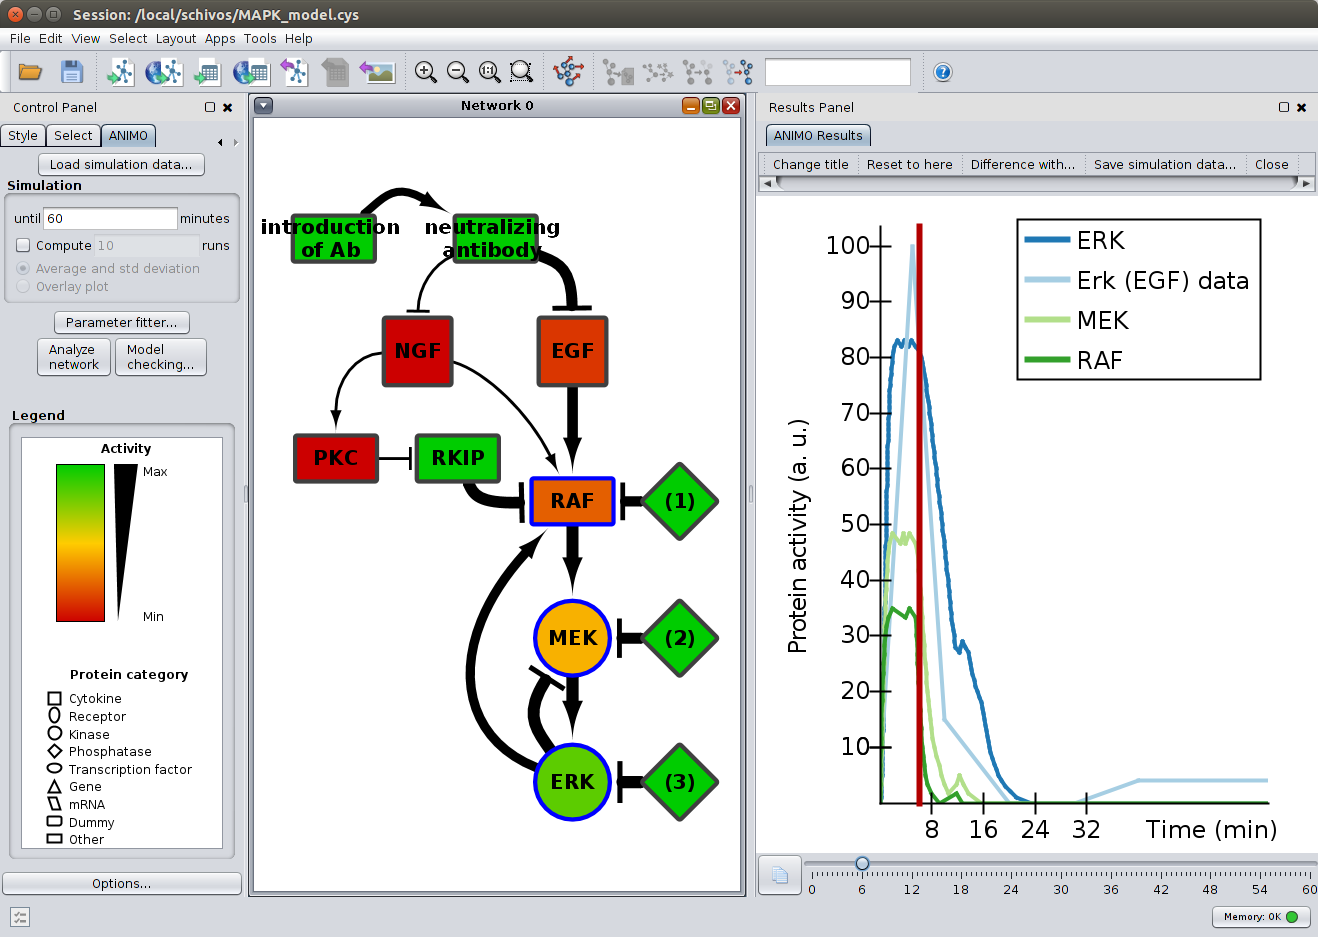
\includegraphics[width=.7\textwidth]{images/ANIMO3_MAPK_model} %mapk_model_egf4}
\end{center}\vspace{-.5cm}
\caption{The Cytoscape 3 user interface running the new ANIMO app
(model from~\cite{animo-ieee}). The \emph{Network} panel in the center contains the nodes-edges
model of the cross-talking signaling pathways of NGF and EGF, with
colors indicating node activity levels and shapes representing different protein categories (see the \emph{Legend} on the left).
The \emph{Results Panel} on the right contains a graph plotting activity levels of selected nodes
during the first hour of evolution of the model. The slider under the graph
allows the user to select the time instant (marked as a vertical red line in the graph) on which
the colors nodes in the \emph{Network} are based. The edge thickness is used to give an idea on which reactions are
occurring more often at the selected time instant.
The series {\sf Erk (EGF) data} in the graph is the experimental
data from~\cite{egf-ngf} for the 100~ng/ml EGF treatment.
\label{fig:cytoscape}}
\vspace{-.5cm}
\end{figure}

We consider a \emph{molecular species} (also called \emph{reactant}) to include all the molecules of the same substance in both their active
and inactive state inside the cell. In order to distinguish between the two activity states in which each molecule can be,
we define the \emph{activity level}
to represent the percentage of active molecules over an entire molecular species. In an ANIMO model, this value
is discretized on a given integer interval, to adapt to the quality
of available experimental data and (for large models) allow for a trade-off between performance and precision.
The user can choose the granularity for each molecular species separately, on a scale between 2 (the
reactant is seen as either completely inactive or completely active) and 101 levels (allowing to represent activity as $0, 1\%, 2\% \dots\ 100\%$).
The activity level of a molecular species is represented in the ANIMO network
by coloring the corresponding node according to the scale shown in the {\sf Activity} legend in Figure~\ref{fig:cytoscape},
where the minimum indicates that all molecules of the given species are inactive.

The occurrence of a \emph{reaction} modifies by one discrete step the activity level of its target reactant, making it increase or decrease 
depending on whether the reaction is defined, respectively, as activating or inhibiting.
The rate with which a reaction occurs depends on a formula selected by the user. 
Choosing one of three available scenarios allows the user to make the reaction rate depend on
the activity of one or two reactants.
The rate of each reaction can be scaled by modifying the value of one kinetic constant $k$,
possibly using a qualitative measure from a predefined set ({\sf very slow}, {\sf slow},
{\sf medium}, {\sf fast}, {\sf very fast}).
% Approximating the actual reaction dynamics with less detailed single-parameter scenarios
% leads to a kinetic model that is still precise enough to faithfully represent the behavior of a signaling network.
The approximation allows us to reduce the dependence of a model from often unavailable quantitative
parameters for biochemical reaction kinetics, while keeping a precision level that is still precise enough to be useful.
For a more precise dissertation on how reaction rates are computed in ANIMO, we recommend~\cite{animo-ieee},
where the previously used \tas\ model is presented. The reader interested in the current
methods for parameter setting in ANIMO can refer to~\cite{animo-syncop}.




\section{A new way of modeling signaling pathways with \tas}\label{sec:animo-new}
We present here a novel model to represent signaling pathways with \tas\ in ANIMO.
We define the model previously used in ANIMO to be \emph{reaction-centered}, as for each reaction
in the network an instance of a \ta\ template is generated to mimic
the occurrences of that reaction. Observing that signaling
networks tend to be highly connected, containing noticeably more reactions than reactants,
we shift the focus on reactants instead, achieving what we call a \emph{reactant-centered} model.
This change of view is inspired by the classical way in which biological events are modeled
with ordinary differential equations (ODEs)~\cite{ode-ma-anche-altro}.

% \begin{figure}
%   \centering
%   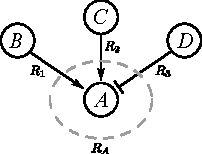
\includegraphics[width=0.3\textwidth]{images/network_abcd}
% \caption{A signaling network where one node is influenced by three distinct reactions.
% The (virtual) reaction $R_A$ is defined in the reactant-centered model
% as the algebraic sum of the reactions influencing $A$.
% % The reaction-centered ANIMO model from~\cite{animo-ieee} would generate three
% % \tas, while the model presented here would lead a single automaton representing $R_A$.
% }\label{fig:network-abcd}
% \end{figure}


\subsection{The reactant-centered approach}\label{sec:reactant-centered}
The reactant-centered model presented here is based on the concept of \emph{net effect} of a set of reactions on a reactant:
instead of considering each reaction in isolation, we consider their combined influence on each reactant.
As an example, consider a reactant $A$ activated by reactions $R_1$ and $R_2$, and inhibited
by reaction $R_3$ (see Fig.~\ref{fig:network-abcd}).
The net effect of these three reactions on $A$ defines the \emph{net reaction} $R_A = R_1 + R_2 - R_3.$
Applying a concept similar to the definition of an ODE,
where the rate of change of each reactant depends on the rate of the reactions influencing it,
the rate of $R_A$ is computed as the sum of the rates of the reactions influencing~$A$: 
$$r_A = r_1 + r_2 - r_3$$
where $r_i$ is the rate of reaction $R_i$ and is defined as follows.
Consider $R_1$ to be the reaction $B \rightarrow A$ with kinetic constant $k_1$.
Suppose the settings in the ANIMO network for $R_1$ make its rate depend only on the
activity level of $B$. Then we compute the rate of $R_1$ as $r_1 = [B] \times k_1$, with
$[B]$ the current activity level of~$B$.


\def\scalaOldModel{0.25}
\def\reactantTA{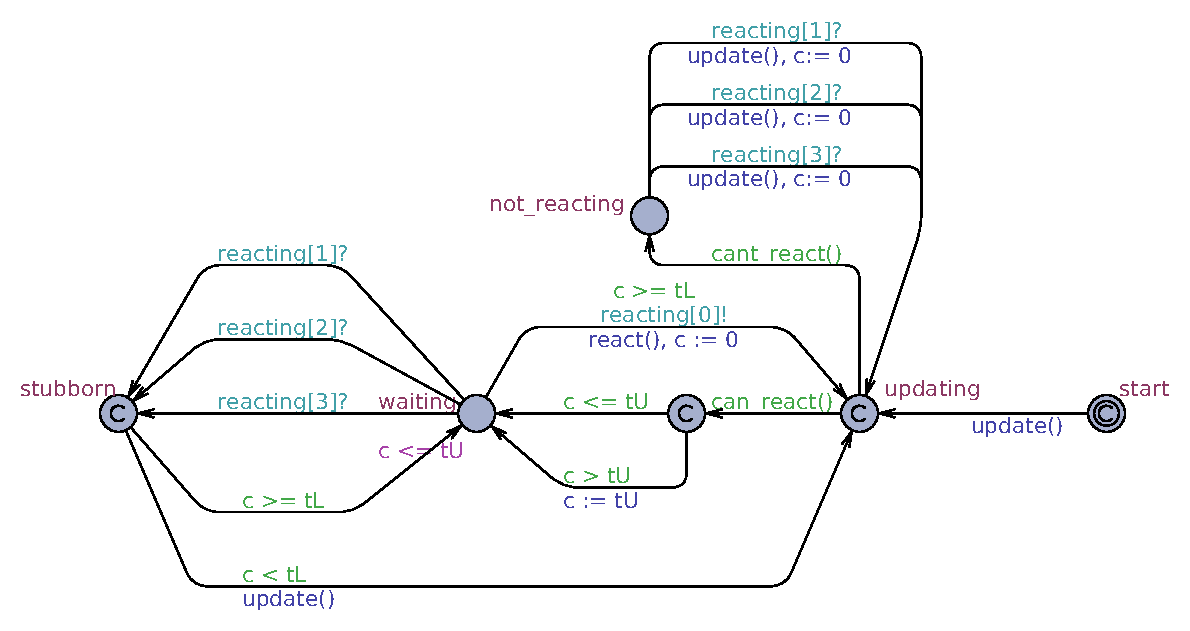
\includegraphics[scale=0.35]{images/Reactant_R3}}
\newlength\reactantTAheight
\setlength\reactantTAheight{\heightof{\reactantTA}}

\begin{figure}[thb]
  \begin{center}
  \subfloat[\label{fig:network-abcd}]{\begin{minipage}[c][\reactantTAheight]{0.26\textwidth}\begin{center}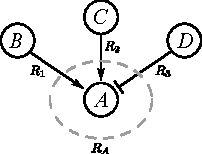
\includegraphics[scale=1.0]{images/network_abcd}\end{center}\end{minipage}} \qquad\qquad\quad
  \subfloat[$R_A$\label{fig:ta-new-model}]{\begin{minipage}[c][\reactantTAheight]{0.6\textwidth}\begin{center}\reactantTA\end{center}\end{minipage}} \\
  \subfloat[$R_1: B \rightarrow A$ \label{fig:ta-old-BA}]{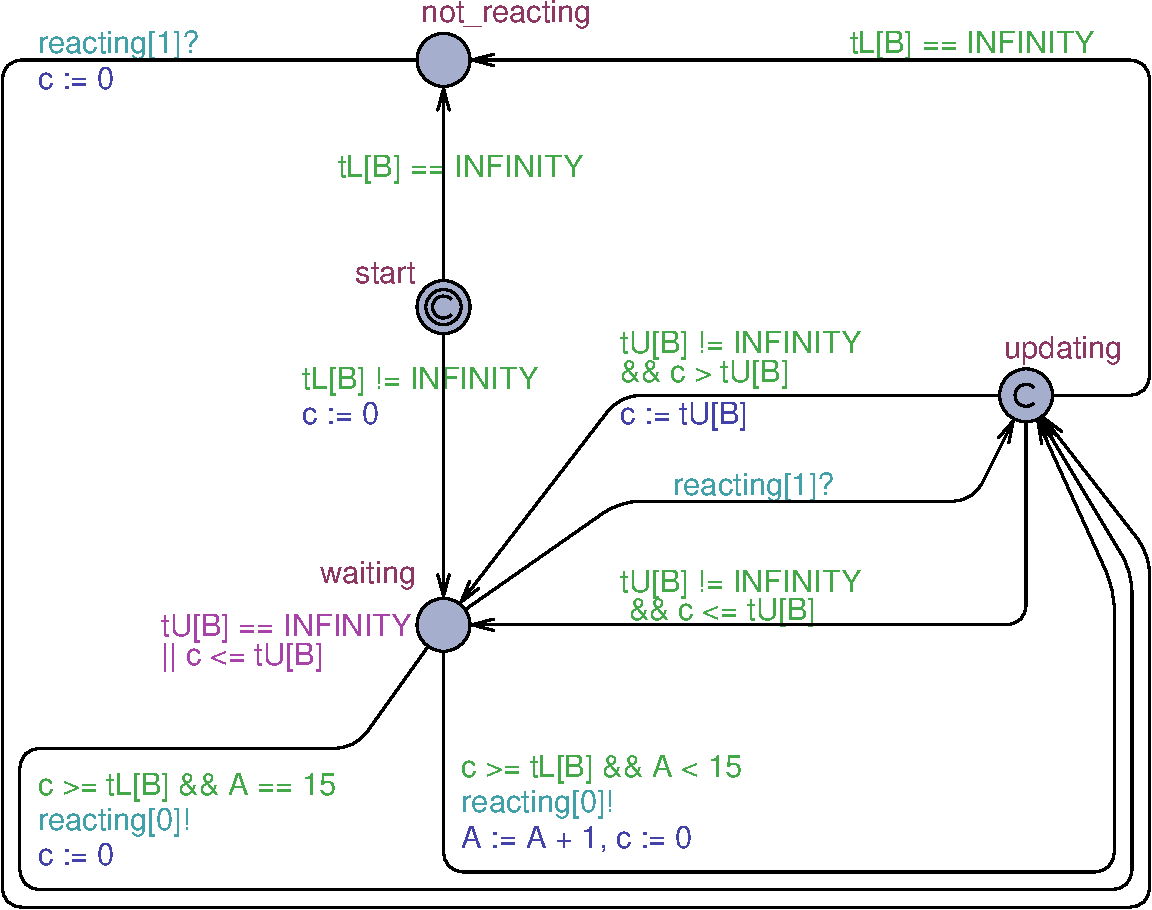
\includegraphics[scale=\scalaOldModel]{images/Reaction_B_A}} \qquad\qquad
%   \subfloat[$R_2: C \rightarrow A$ \label{fig:ta-old-CA}]{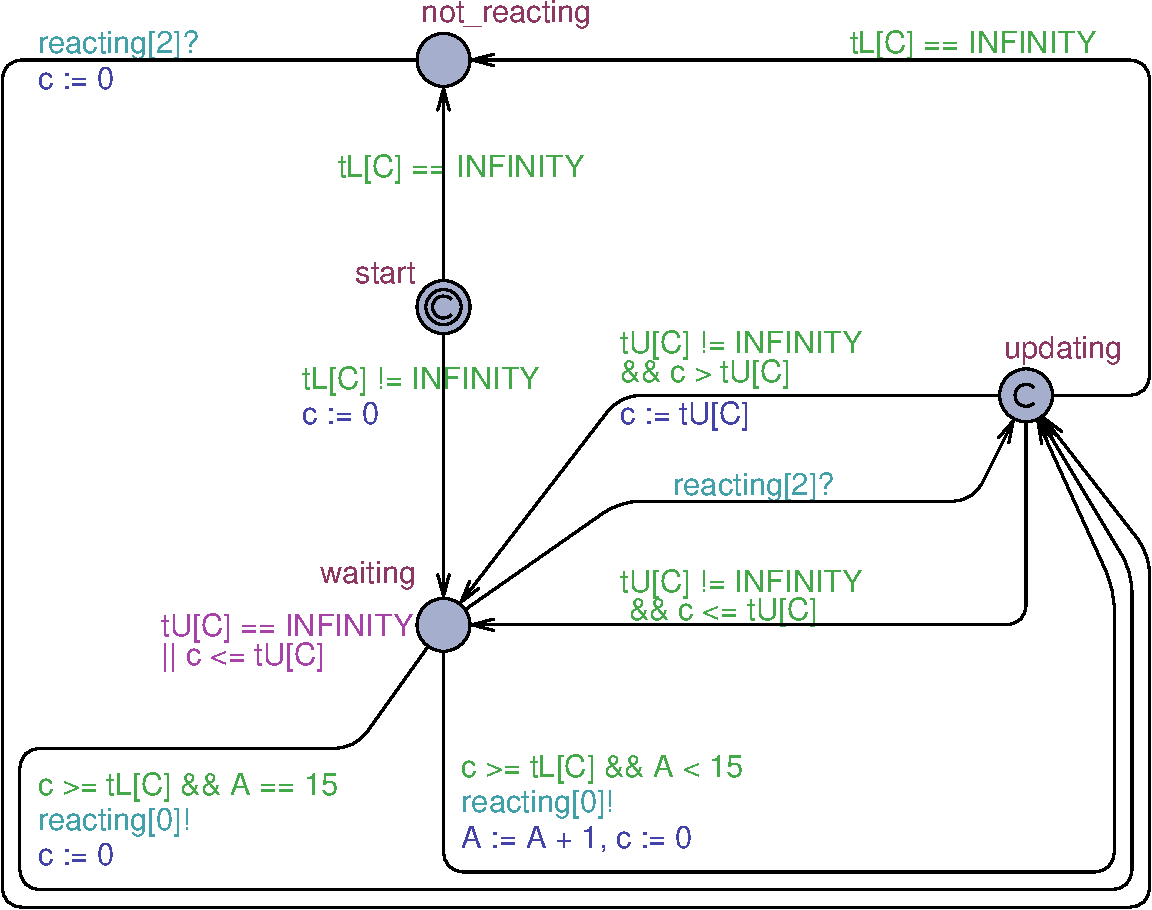
\includegraphics[scale=\scalaOldModel]{images/Reaction_C_A}} \qquad\qquad
  \subfloat[$R_3: D \dashv A$ \label{fig:ta-old-DA}]{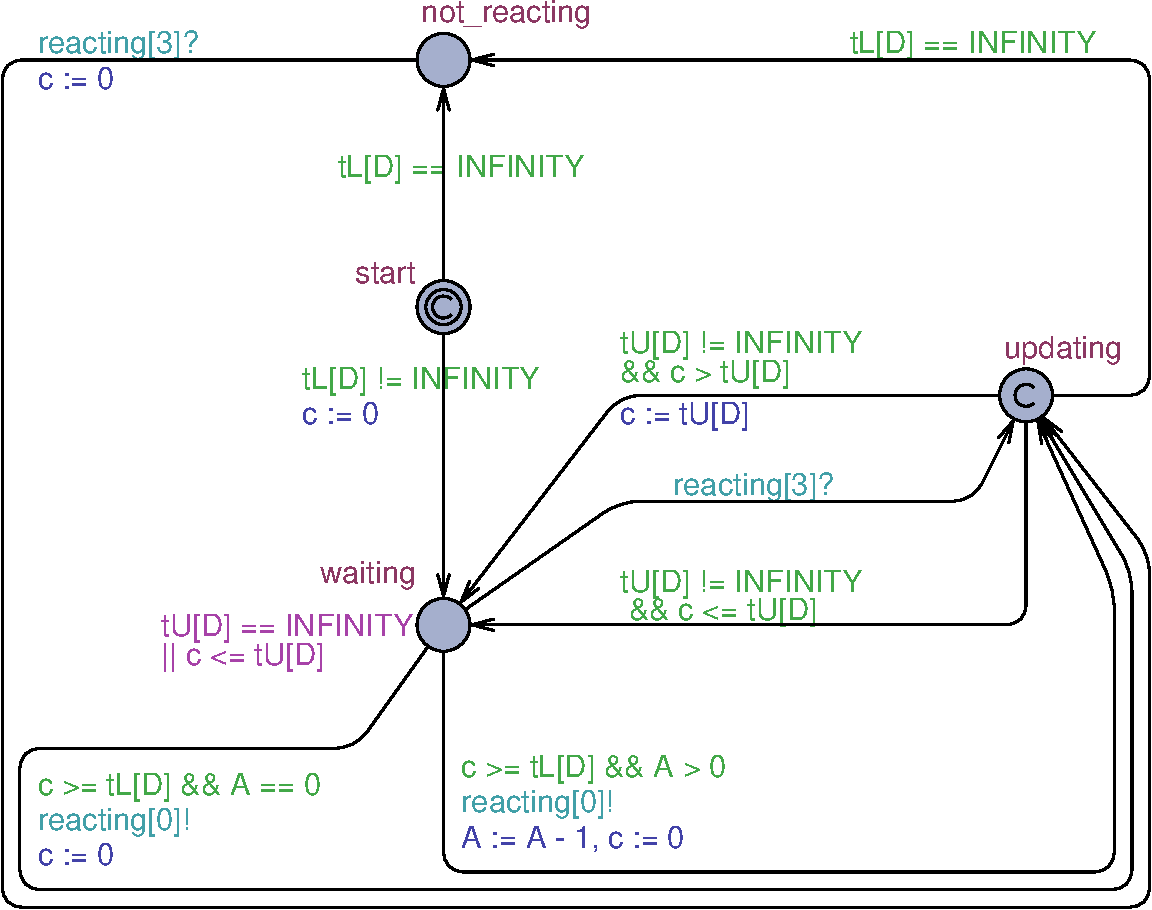
\includegraphics[scale=\scalaOldModel]{images/Reaction_D_A}}
  \end{center}\vspace{-.5cm}
  \caption{
{\bf\protect\subref{fig:network-abcd}} A signaling network where one node is influenced by three distinct reactions.
The (virtual) reaction $R_A$ is defined in
the reactant-centered model as the algebraic sum of the reactions influencing $A$.
({\bf\protect\subref*{fig:ta-new-model}\--{}\protect\subref*{fig:ta-old-DA}}) \tas\ templates generated by ANIMO for the reactant-centered~{\bf\protect\subref{fig:ta-new-model}}
 and reaction-centered~({\bf\protect\subref*{fig:ta-old-BA}\--{}\protect\subref*{fig:ta-old-DA}}) models of the network in~{\bf\protect\subref{fig:network-abcd}}.
The templates have been edited for an easier visual comparison; while the template for $R_2$ ($C \rightarrow A$) is qualitatively identical to the one for $R_1$,
and was left out for the sake of space. Functions {\sf can\_react()} and {\sf cant\_react()}
in~{\protect\subref{fig:ta-new-model}} have the same content as the corresponding guards in ({\bf\protect\subref*{fig:ta-old-BA}\--{}\protect\subref*{fig:ta-old-DA}}),
while function {\sf update()} in~{\protect\subref{fig:ta-new-model}}
replaces the references to the pre-computed tables {\sf tL[]}, {\sf tU[]} with on-the-fly computation (see Sect.~\ref{sec:rates-ta-model}).
% \ta\ template used to represent a net reaction in the reactant-centered model.
\label{fig:ta-models}}
\end{figure}


As with ODEs, if $r_A$ is positive the activity level of $A$ will increase;
otherwise, $A$ will decrease its activity level.
The absolute value of $r_A$ determines the speed with which such change happens.
The value of the reaction rate is thus translated into a time value to be used as
time bound in the \ta\ representing $R_A$ (see Fig.~\ref{fig:ta-new-model}) by computing
$$T_A = \frac{1}{\mbox{abs}(r_a)}$$
with $\mbox{abs}(r_a)$ the absolute value of $r_a$. In order to represent
a natural variability in reaction timing, we relax the exact value of $T_A$ by
defining bounds of~$\pm~5\%$ (which can be changed by the user):
$$
\begin{array}{lcl}
  \mbox{\sf tL} &=& T_A \times 0.95 \\
  \mbox{\sf tU} &=& T_A \times 1.05
\end{array}
$$
Analogously to the reaction-centered model of~\cite{animo-ieee},
we will call {\sf tL} the \emph{lower time bound} and {\sf tU} the \emph{upper time bound}.
Note that here, differently from what presented in~\cite{animo-ieee}, we do not define
pre-computed tables with all possible values for {\sf tL} and {\sf tU}: this is because
the number of variables for the computation of a reaction rate can be arbitrarily high, and
the size of such tables grows exponentially with the number of variables.
In the example of Figure~\ref{fig:ta-models}, a table to represent the time bounds
for reaction ${R_A}$ would have four dimensions, depending on the activity levels
of reactants $A$, $B$, $C$ and $D$. Assuming that all four reactants are discretized
on 101 levels (activity levels from 0 to 100), each of the two tables {\sf tL} and {\sf tU} would contain $101^4 = 104\,060\,401$
elements. Adding one more reaction $E \rightarrow A$ to the pool would make
this approach exceed the memory limits of most of the currently available computers
% , requiring about 78 gigabytes of memory to be stored.
For this reason, the reaction rates are computed on the fly (see Section~\ref{sec:rates-ta-model}).


\subsection{Timed Automata reactant-centered model}\label{sec:ta-model}
The behavior of the \ta\ representing the net reaction $R_A$ is defined as follows: after a number of seconds
variable inside the continuous interval $[\mbox{\sf tL}, \mbox{\sf tU}]$ (measured with the local clock {\sf c}),
the activity level of $A$ will increase or
decrease by one step, depending on the sign of $r_A$; then new values for $r_A$, {\sf tL} and {\sf tU} will be computed based
on the (possibly) changed conditions.

The process described in Section~\ref{sec:reactant-centered} to compute the values of {\sf tL} and {\sf tU} is an instance of the function called {\sf update()}
in the \ta\ template of Figure~\ref{fig:ta-new-model}. The computation of {\sf update()} is the first step
taken when initializing a new model taking the transition from the initial location {\sf start} (identified by two concentric circles)
to {\sf updating}.
Location {\sf updating} is then used to decide whether $R_A$ can be executed or not (functions
{\sf can\_react()} and {\sf cant\_react()} used as guards for the transitions exiting from {\sf updating}).
This decision is based on the computed value for
$r_A$ and the current activity level of $A$: if $r_A > 0$ and $A$ is already completely active
(or  $r_A < 0$ and $A$ is completely inactive), no
update to $A$ can be applied, so the automaton switches to location {\sf not\_reacting}.
Moreover, $r_A$ can be $0$: this means
that the reactions influencing $A$ balance each other to complete cancellation, so also in this
case $R_A$ cannot occur and the next location will be {\sf not\_reacting}. Otherwise (i.e. if {\sf can\_react()} is true), the activity
level of $A$ can be changed, so the next location will be the one labeled {\sf waiting}, which
is reached after having made sure that its clock invariant is respected (committed location
between {\sf updating} and {\sf waiting}).

When in location {\sf waiting}, the local clock {\sf c}
is let run until enough time has passed for the reaction to occur: this is obtained by using {\sf c $>=$ tL} as guard
for the transition from {\sf waiting} to {\sf updating}.
Because of the invariant {\sf c $<=$ tU} on {\sf waiting}, we ensure that the reaction occurs after no more than {\sf tU} seconds have passed.
The transition to {\sf updating} leads to an update to the activity level of $A$ (call to {\sf react()}), together with the computation of new values for $r_A$,
{\sf tL} and {\sf tU} (function {\sf react()} calls {\sf update()}). Moreover, we see in Figure~\ref{fig:ta-new-model}
that a communication is sent on channel {\sf reacting[0]} ($0$ is the index
assigned to reactant $A$): this is used to warn
the other automata that the activity level of $A$ has just changed, possibly changing the conditions for
other reactions.

On the other hand, one of the reactants influencing a reaction on which $A$ depends may change its activity level
before $R_A$ can occur: this event may have an influence on the value of $r_A$, so a re-computation
of $r_A$, {\sf tL} and {\sf tU} is needed.
In the template of Figure~\ref{fig:ta-new-model}, the indexes of the influencing reactants are 1, 2 and 3,
corresponding respectively to $B$, $C$, $D$ in Figure~\ref{fig:network-abcd}.
Whenever a communication on one of the channels corresponding to an influencing
reactant is received while in location {\sf waiting}, the automaton moves to location
{\sf stubborn}. This location was introduced to avoid unwanted non-deterministic behavior\footnote{The term \emph{unwanted}
refers to a non-determinism that is not related to actual biological concepts, but to the semantics of the modeling
paradigm.} in the model.
In the example, this could happen when the activity level of $B$ is updated concurrently (in the same instant) with the activity level of $A$.
As $B$ influences $A$ through reaction $R_1$, any change in the activity level of $B$ causes a change in $r_1$, thus
requiring a recomputation of $r_A$, {\sf tL} and {\sf tU}. Due to the interleaving nature of \tas\ semantics, only one automaton
may change location for the \tas\ system to change state. This means that, should the activity level of $B$ be changed
first, the conditions for $R_A$ would be recomputed, possibly preventing the update to $A$ to occur. Vice versa, should the activity
level of $A$ be changed first, both $A$ and $B$ could change their activity levels.
In such a situation, the non-deterministic order in which the updates are computed decides the behavior of the model.
To avoid this, we ensure that if a reaction can occur in a given instant (i.e. {\sf c $>=$ tL}), it will not
consider the concurrent updates to influencing reactants (in the example, having the clock reach {\sf tL} ensures that $R_A$ occurs,
independently from any concurrent update to $B$).
Performing a check on the current value of the clock {\sf c} with respect to the reaction lower time bound allows
an automaton to detect the case of a concurrent update, remaining ``stubborn'' in its resolution
of reacting with the current configuration: the guard {\sf c $>=$ tL} on
the transition returning from {\sf stubborn} to {\sf waiting}
is the same as the guard on the transition from {\sf waiting} to {\sf updating} and
implies that the transition could occur in the current time instant.
If no conflict is found, i.e. {\sf c $<$ tL}, a new time limit for the reaction is
computed via function {\sf update()} while moving to location {\sf updating}. Note that the clock {\sf c} is not reset
when moving from {\sf stubborn} to {\sf updating}: should the new conditions only change the value of {\sf tL} and {\sf tU}
without disabling the reaction, the ``partial work'' of the reactions is not discarded.

Finally, location {\sf not\_reacting} is used to avoid reacting when not necessary (see the description
of {\sf cant\_react()} above), and to respond to changes in those reactants
which can influence the value of $r_A$. Should one of such reactants change its activity level, the
conditions are updated and the local clock is reset, moving to {\sf updating} to check whether the reaction can now
occur.

\subsection{Computations on the fly}\label{sec:rates-ta-model}
Reaction rates are all computed at run-time by the function {\sf update()},
and are based on the user-chosen scenarios, their kinetic constant $k$ and the activity level of the involved reactants.
As such computations require floating-point precision but UPPAAL only provides integer
variables and operators, we use a significand-and-exponent notation with 4 significant figures, which allows for an error
in the order of $0.1 \%$ while 
avoiding integer overflow in UPPAAL's engine.
For example, the floating point number $a = 1.23456$ will be represented as the pair $\langle 1235, -3 \rangle$,
which is translated back as $a = 1235 \times 10^{-3} = 1.235$.
% As an example of such a notation, consider the two floating-point numbers
% $a = 1.23456$ and $b = 0.00023456$, and their sum $c = a + b = 1.23479456$. The corresponding representations in
% our integer-based notation will be:
% $$
% \begin{array}{rcl}
%   a = \langle 1235, -3 \rangle &=& 1235 \times 10^{-3}\\
%   b = \langle 2346, -7 \rangle &=& 2346 \times 10^{-7}\\
%   a + b = \langle 1237, -3 \rangle &=& 1237 \times 10^{-3}
% \end{array}
% $$
% In this case, the number representing the sum $a + b$ differs from the exact result by $c - 1237 \times 10^{-3} = 0.001456$.
The interested reader can find the UPPAAL definitions and functions needed to compute rate and time values for the \tas\ templates
% in Appendix~\ref{apx:double-functions} or 
inside any UPPAAL model file generated by ANIMO with a reactant-centered model type~\footnote{Models generated
by ANIMO are saved in the system's temporary directory. Further details are available in
the ANIMO manual at \url{http://fmt.cs.utwente.nl/tools/animo/content/Manual.pdf}}.


\subsection{Comparison with the previous \tas\ model}\label{sec:ta-notes}
% A qualitative parallel between the reactant- and reaction-centered versions of the \tas\ model
% can be made by intuitively matching locations with the same name on the two models.
With reference to Figures~\ref{fig:ta-new-model} and~\ref{fig:ta-models}{\protect\subref*{fig:ta-old-BA}\--{}\protect\subref*{fig:ta-old-DA}},
we propose a qualitative parallel between the reaction- (old) and reactant-centered (new) \tas\ models.
The first remark is that equally-named locations have the same function in the automaton: so for
example location {\sf waiting} is used to wait before updating the reactant.
% The central location is in both cases labelled {\sf waiting}: there the automaton waits
% until the time has come for the reaction to occur. The amount of time to be waited has different meanings:
% in the reaction-centered model, 

Being based on the same abstractions, the two models can be analyzed with the same
UPPAAL queries for all the cases for which biology is involved. The differences can be seen only if the
analysis focuses on the single automaton level and explicitly refers to locations: such type of analysis
is normally not necessary when considering the model as a whole and using it for what it is, i.e. an
abstract representation of a set of biological processes.

We note that replacing all the existing reactions with the net reactions relative to each
reactant in a model does change the behavior of the model in the sense that continuous oscillations
of activity levels around an equilibrium point are less frequent. However, this does not mean that the
behavior of two models using the two different approaches will diverge: the equilibrium points
are still the same.
Two opposite reactions occurring with the same (or similar) frequency will (nearly) cancel each other out: the
behavior of the single reactions is explicitly represented in the reaction-centered model and gives rise to more oscillations.
On the other hand, in the reactant-centered model, the trajectory of a reactant's activity level
is determined taking into account also the canceling effect of opposite reactions, so the simulations
will generally contain less oscillations.
From the user's point of view, graphs will look smoother while still exhibiting the same qualitative behavior,
as can be seen in Figure~\ref{fig:comparison-graph-animo}.
The \tas\ templates in Figure~\ref{fig:ta-models} show that the main difference between the two approaches
is indeed due to the choice of lumping all the reactions influencing $A$ into the single
reaction $R_A$.
% Exhibiting less oscillations means generating less events (i.e. changes of state) in the underlying \tas\ model, as in both approaches each change
% in reactant activity level is caused by an event in the \tas\ model. Less events means smaller state spaces, thus lower analysis times.
In the next session we will show that having less oscillations leads in practice to better analysis performances.
\begin{figure}[!htb]
\begin{center}
  \subfloat[Reaction-centered]{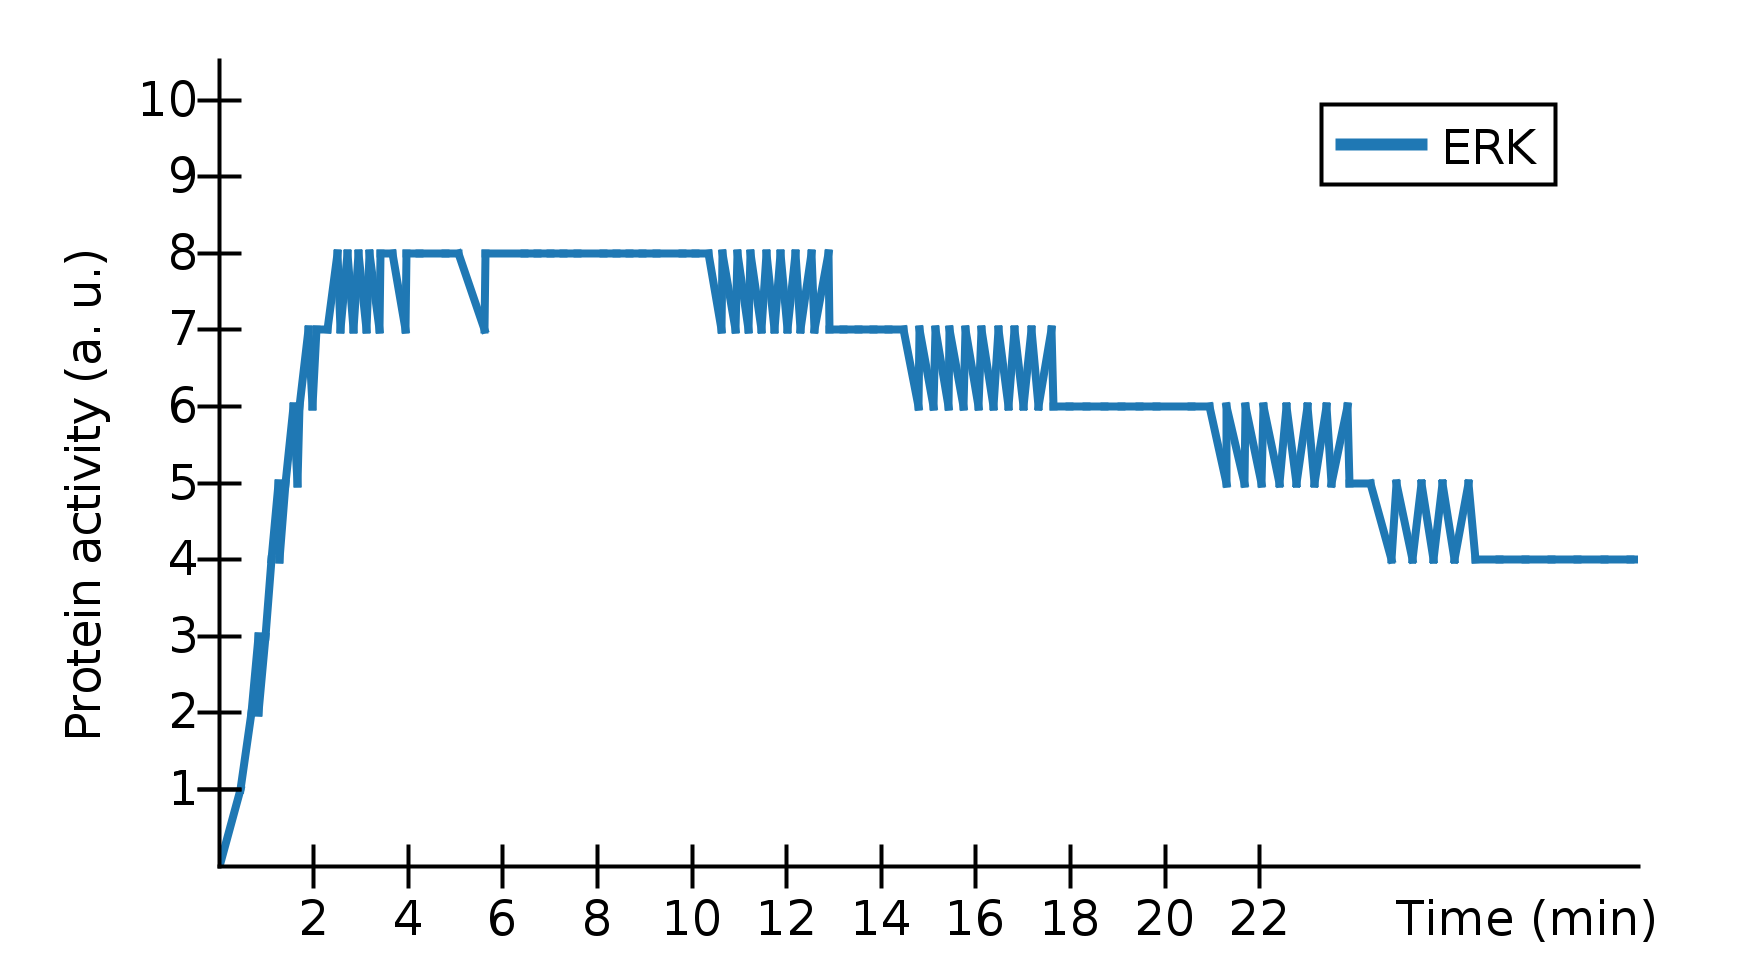
\includegraphics[scale=0.07]{images/grafico_ngf_reaction_10levels}\label{fig:comparison-graph-animo-reaction}}\qquad\qquad
  \subfloat[Reactant-centered]{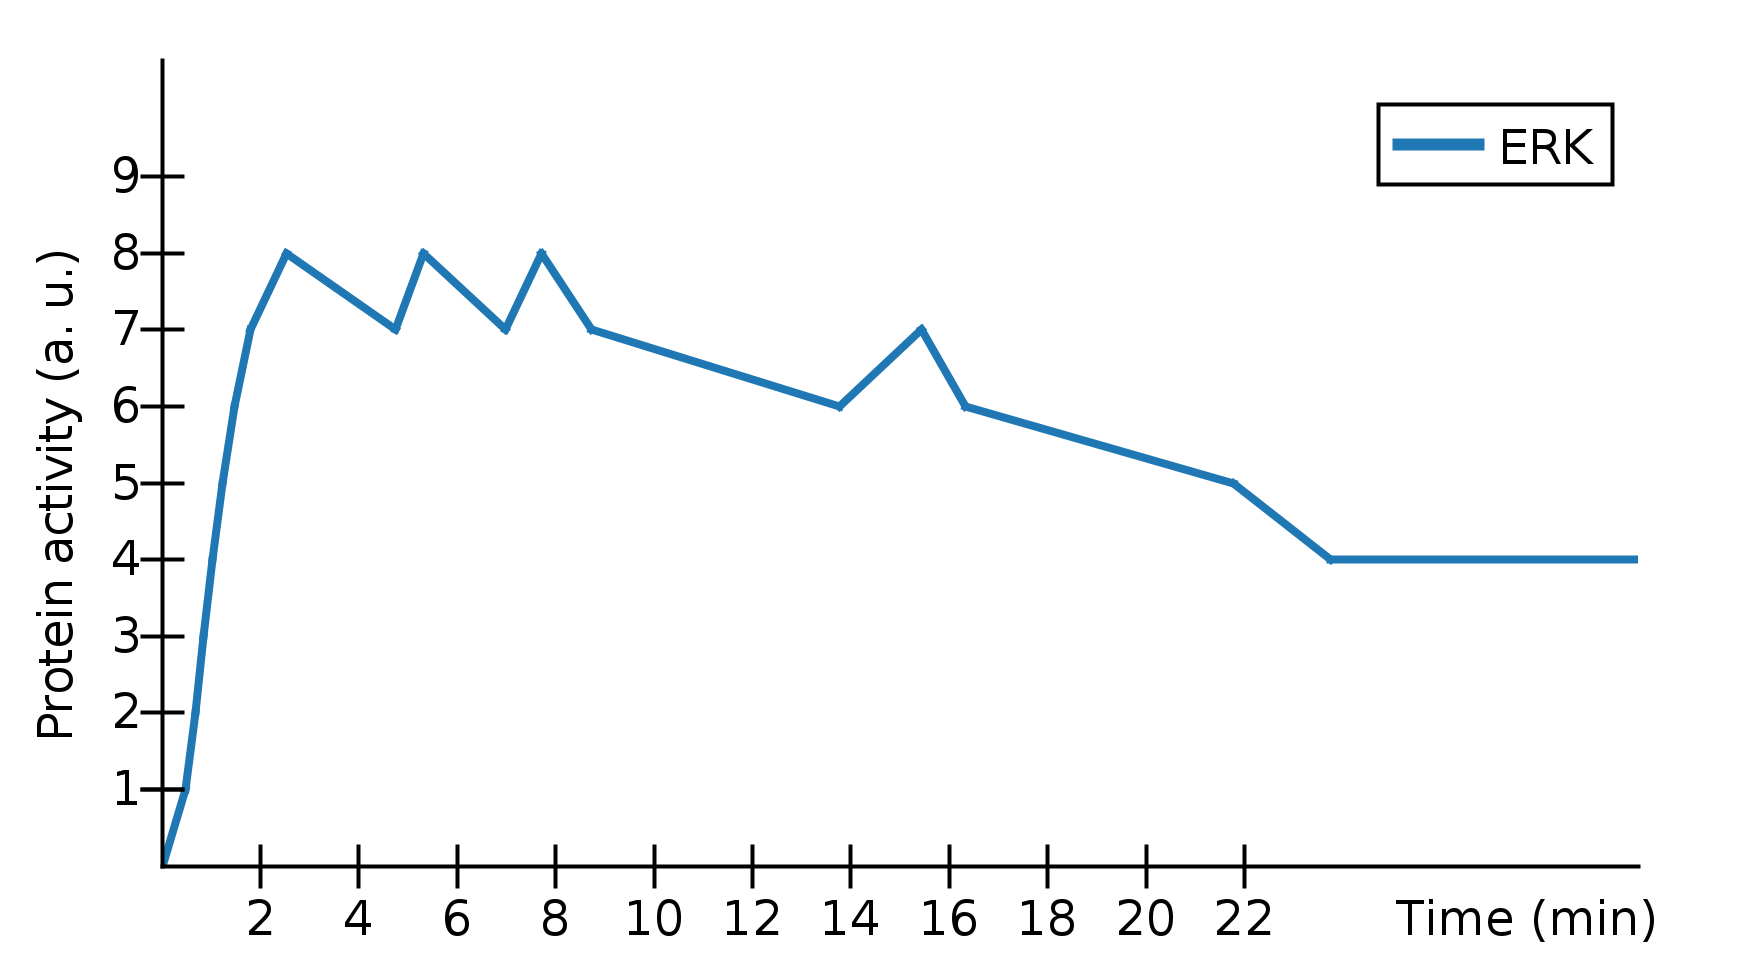
\includegraphics[scale=0.07]{images/grafico_ngf_reactant_10levels}\label{fig:comparison-graph-animo-reactant}}
\end{center}\vspace{-.5cm}
  \caption{Comparison of two ERK activity graphs generated from the model based on the case study from~\cite{animo-ieee} with treatment of 50 ng/ml NGF.
  ERK was set to 10 levels of granularity to evidence the oscillations in the graphs.
  \label{fig:comparison-graph-animo}}
\end{figure}


\section{Reaction-centered VS reactant-centered}\label{sec:animo-comparison}
We will now apply some basic model checking queries to the case study presented in~\cite{animo-ieee},
measuring the performances of the two modeling approaches. This will allow us to
evaluate the benefit brought by the shift in perspective from a reaction- to a reactant-centered model.

All experiments were carried out on an Intel\circledR\ Core$^{\mbox{\scriptsize\texttrademark}}$ i7 CPU at 2.80GHz equipped with 4 Gb RAM
and running Ubuntu GNU/Linux 14.04.1 64bit.
UPPAAL version 4.1.19 64bit was used to compute the result of the queries, asking for ``some trace'' with random depth-first search order
when an execution trace was expected to be produced. For the simulation queries using the statistical model checking engine, we left
all options at their default values.

The case study we use as a testbed is the network model shown in the \emph{Network} panel in Figure~\ref{fig:cytoscape},
which represents signaling events downstream of growth factors EGF (epidermal growth factor)
and NGF (nerve growth factor) in PC12 cells (a cell line used to study neuronal differentiation).
The model topology proposed in~\cite{egf-ngf} was analyzed
with an ANIMO model based on the reaction-centered approach, reproducing the experimentally 
observed ERK (extracellular signal-regulated kinase) activity changes~\cite{animo-ieee}.
In particular, a 10 minutes stimulation with EGF resulted in transient behavior (i.e. peak-shaped,
see also the graph in Fig.~\ref{fig:cytoscape}), while NGF stimulation led to sustained activity (see Fig.~\ref{fig:comparison-graph-animo}).

\subsection{Simulation cost}
We start by evaluating the cost of simulation with the two different models. This is a particularly
important aspect to consider, as during the model building phase a user may need to perform a large number of simulations,
continuously adapting the topology or quantitative parameters of a network model. In order to make
the modeling approach in ANIMO as interactive as possible, it is desirable to decrease dead times,
and this translates into reducing the computational cost of model analysis as much as possible.
UPPAAL's statistical model checking engine~\cite{uppaal-smc} is based on the generation of random walks (i.e., simulation runs) from a \tas\ model.
In this experiment, we query UPPAAL for simulation runs on the models
generated by ANIMO applying the reaction- and reactant-centered modeling approaches to the case study.
To define the initial state of the model, we consider the starting condition to be the treatment with 50~ng/ml NGF, which translates into
setting the activity level of node NGF to 15/15, while changing EGF to be at 0/15 activity.
% We have chosen this configuration as the
% model is expected to continue reacting indefinitely (sustained ERK activity), without reaching a deadlock state where all reactions are inactive.
% This makes the model more demanding when generating the state space
% because having more reactions occur means having more states in the transition system underlying the \tas\ model.
This configuration was chosen as it generates a more interesting behavior from the biological point of view,
also w.r.t. the model checking queries in Section~\ref{subsec:model-checking-performances};
the treatment with 100~ng/ml EGF was also tested and gave similar performance results.
Table~\ref{tab:sim-100} illustrates the computation time and memory usage when performing 100 simulation runs on each of the
two considered models. Computing the simulation runs took about $91 \%$ less time with the reactant-centered model, using $97 \%$
less memory. This decrease in computation time for long simulation runs brings the approach nearer to the idea
of interactive exploration of a network.

\begin{table}
  \begin{center}
  \begin{tabular}{|l||r|r|}
    \hline
    Model type & Time (s) & Memory (peak KB) \\
    \hline
    \hline
    Reaction-centered & 30.72 & 291\,{}576 \\ %37.14 & 257,928 \\
    \hline
    Reactant-centered & 2.86 & 9\,{}768 \\ %2.83 & 33,464 \\
    \hline
  \end{tabular}
  \end{center}
  \caption{UPPAAL processor time and memory usage for reaction- and reactant-centered modeling approaches when computing
  the query {\tt simulate 100 [36000] \{ R1, R2, \dots, R11 \}} on the model from~\cite{animo-ieee} with starting condition
  NGF = 15/15, EGF = 0/15, corresponding to a treatment with 50 ng/ml NGF.
  The query asks for 100 time series of the activity levels of all reactants in the model over the first 60 minutes
  of execution.\label{tab:sim-100}}
\vspace{-1cm}
\end{table}

\subsection{Model checking performances}\label{subsec:model-checking-performances}
Next, we set out to test the model checking performances on the two versions of the \tas\ model, comparing the
execution times and memory requirements for a number of interesting queries:
\begin{itemize}
  \item (1) and (2): {\tt A[] not deadlock}. The model continues to execute indefinitely ({\tt []} refers to all
      possible paths in the transition system of the model, and {\tt A} asks the property to always hold along a path).
  \item (3): {\tt RKIP $<$ 10 --$>$ ERK $>=$ 40}. After RKIP (Raf kinase inhibitory protein) activity has been lowered, ERK activity increases. As in the model RKIP
      has 20 levels of granularity and ERK has 100 levels, {\tt RKIP $<$ 10} means that RKIP is less than half active, and
      {\tt ERK $>=$ 40} means that ERK activity is at least $40 \%$.
  \item (4): {\tt E<> RKIP $<$ 10}. Find a point when RKIP is low ({\tt <>} asks for the existence of at least one path
      for which the property holds, while {\tt E} requires the property to hold at least once in a given path).
      This query is expected to generate a trace, the last point of which will be used as initial configuration for model checking queries (5) and (6).
  \item (5): {\tt A[] ERK $<$ 70} and (6): {\tt A[] ERK $>$ 35}. Once RKIP activity has significantly decreased, ERK activity is sustained at an intermediate level.
\end{itemize}
The initial conditions are:
\begin{itemize}
  \item (1): EGF = 15/15 and NGF = 0/15, all others as the original configuration, corresponding to the treatment condition with
	    100 ng/ml EGF.
  \item (2) - (4): EGF = 0/15, NGF = 15/15, all others as the original configuration, corresponding to the treatment condition with
	    50 ng/ml NGF\footnote{In the laboratory experimental setting, NGF is used at a lower concentration than EGF, but it is still enough to saturate all NGF receptors, which
	    are rarer than EGF receptors.}.
  \item (5) and (6): all activities as in the last state of the trace computed from query~(4).
\end{itemize}

We note that performing model checking means dealing with state space explosion problems,
and model reduction is recommendable in order to obtain any result within adequate time limits. One of the
most user-accessible ways available in ANIMO to reduce the size of a model is setting the uncertainty to 0
before performing model checking queries.
In order to still consider some biological variability, the user can manually perform multiple model checking queries with changed interaction parameters.
The tests performed in this section have an uncertainty level set to 0, instead of the $5\%$ recommended for simulation-based experiments, to
make model checking feasible within seconds.


\begin{table}[htbp]
  \begin{center}
    \begin{tabular}{|c||r|r||r|r||r|r|}
      \hline
       \multirow{3}{*}{Query} & \multicolumn{2}{c||}{Reaction-centered}	   & \multicolumn{2}{c||}{Reactant-centered} & \multicolumn{2}{c|}{Improvement}\\
      \cline{2-7}
       & \multicolumn{1}{c|}{Computation} & \multicolumn{1}{c||}{Memory usage} & \multicolumn{1}{c|}{Computation} & \multicolumn{1}{c||}{Memory usage} & \multicolumn{1}{c|}{Time} & \multicolumn{1}{c|}{Memory} \\
       & \multicolumn{1}{c|}{time (s)}    & \multicolumn{1}{c||}{(peak KB)}    & \multicolumn{1}{c|}{time (s)} & \multicolumn{1}{c||}{(peak KB)} & \multicolumn{1}{c|}{(n-fold)} & \multicolumn{1}{c|}{(n-fold)}\\
      \hline
      \hline
      (1) & 126.56 & 523\,{}448 & 1.04 & 9\,{}236 & 122 & 57 \\ %127.25 & 351\,{}804 & 1.42 & 25\,{}716 & 90 & 14 \\
      \hline
      (2) & 159.29 & 436\,{}496 & 1.73 & 11\,{}480 & 92 & 38 \\ %167.64 & 269\,{}932 & 1.93 & 26\,{}112 & 87 & 10 \\
      \hline
      (3) & 146.09 & 439\,{}484 & 1.04 & 10\,{}384 & 140 & 42 \\ %150.90 & 318\,{}460 & 1.44 & 26\,{}136 & 105 & 12 \\
      \hline
      (4) & 0.74 & 293\,{}508 & 0.06 & 7\,{}484 & 12 & 39 \\ %2.15 & 216\,{}920 & 0.11 & 25\,{}316 & 19 & 9 \\
      \hline
      (5) & 581.79 & 448\,{}764 & 6.86 & 16\,{}880 & 85 & 27 \\ %470.56 & 311\,{}568 & 2.22 & 26\,{}648 & 212 & 12 \\
      \hline
      (6) & 561.01 & 449\,{}248 & 6.42 & 15\,{}852 & 87 & 28 \\ %453.90 & 357\,{}980 & 2.23 & 26\,{}652 & 204 & 13 \\
      \hline
    \end{tabular}
  \end{center}
  \caption{UPPAAL processor time and memory usage for reaction- and reactant-centered modeling approaches when computing
  the given queries on the case study from~\cite{animo-ieee}.\label{tab:model-checking}}
\vspace{-.5cm}
\end{table}

The queries were used with both the reaction- and reactant-centered \ta\ models,
and returned the same results as expected: in particular, query (1) returned false and all other queries returned true.
From the biological point of view, the answer to query (1) confirms that under EGF treatment no other activity is observed in the model after the initial peak,
while query (2) confirms that with NGF activity continues indefinitely.
Moreover, queries (3) - (6) confirm the result of the simulations shown in~\cite{animo-ieee}, with NGF treatment leading to sustained ERK activity.

The results of the model checking performance test are shown in Table~\ref{tab:model-checking}.


\subsection{Analysis of the results}
% Note that we focus most of our attention on the NGF treatment, as with this configuration the model
% was hypothesized to keep reacting permanently (sustained ERK activity). The results from queries (1) and (2)
% show that this is indeed the case, as EGF treatment leads to all reactions dying out after a number of steps (i.e., deadlock due to all
% automata being in the {\sf not\_reacting} location).
% This means that the queries (3) - (6) deal with a larger state space, leading to presumably lower model checking performances.
Requesting a full inspection of the state space
as we do when using a query of the type {\tt A[]$\phi$} returning true in cases (5) and (6), allows us to indirectly compare the state space size of the two
model versions. As the computation time improvements in Table~\ref{tab:model-checking} show, the reactant-centered model produces
indeed a noticeably smaller state space, allowing for a higher level of interactivity also when performing non-trivial model checking.
Moreover, our experiments point out that the reactant-centered approach considerably lowers the memory
requirements for the model. This is not only due to the absence of possibly large precomputed time tables,
which can contain thousands of elements each.
% \footnote{In the reaction-centered model, having a reaction depend on two 101-levels reactants
% leads to the generation of two time tables containing $101 \times 101 = 10\,{}201$ elements each.}
Indeed, this point was further investigated by implementing a reaction-centered model which
avoids the use of tables and instead makes on-the-fly computations of the time bounds with the same number representation as in the reactant-centered model.
This resulted in improved performances in the cases of reachability and simulation-based queries, with memory requirements closer to the ones for
the reactant-centered model (0.69 s and 24\,{}796 KB for query (4)). However, in all other cases a much larger amount of memory (around 2 Gb) was used
with respect to the table-based implementation of the same model, without leading to appreciable benefits in terms of execution time:
in some cases performances were noticeably deteriorated (600-800 s for queries (1)-(3)).
% These findings support the intuitive idea that a reactant-centered approach
% leads in general to fewer events in a model, and to a smaller state space.
These findings seem to support the idea that a reactant-centered models
have a smaller state space.

Note that while the network we consider for the case study is not particularly large, the gain in performances is still considerable
and promising in the perspective of analyzing more complex networks.



\section{Model checking in ANIMO}\label{sec:animo-model-checking-ui}
In order to allow a non-expert user to profit from the power of model checking, we have implemented
a template-based user interface to define queries directly inside the ANIMO Cytoscape App:
Figure~\ref{fig:model-checking-ui} shows the interface for composing a model checking query in ANIMO.
The mappings between user interface templates and actual model checking queries were inspired
by the ones proposed in~\cite{hidde-templates}, and are shown in Table~\ref{tab:model-checking-templates}.

\begin{figure}[htb]
  \begin{center}
    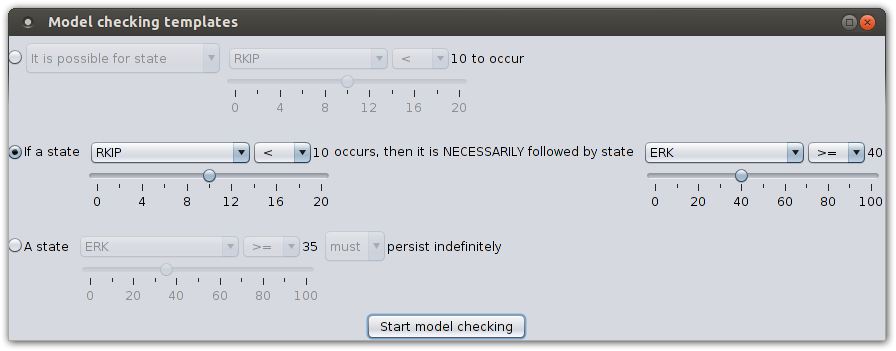
\includegraphics[width=0.7\textwidth]{images/model_checking_ui}
  \end{center}
  \caption{The interface used in ANIMO to compose a model checking query.
  The settings on the three lines correspond, from top to bottom,
  to queries (4), (3) and (6).\label{fig:model-checking-ui}}
\end{figure}

\begin{table}[htb]
  \begin{center}
    \begin{tabular}{|l|l|}
      \hline
      ANIMO template & UPPAAL formula \\
      \hline
      \hline
      It is possible for state $\phi$ to occur & {\tt E<>\hspace{-1.3mm} $\phi$} \\
      \hline
      State $\phi$ never occurs & {\tt E<>\hspace{-1.3mm} !\hspace{-0.5mm}($\phi$)} \\
      \hline
      If a state $\phi$ occurs, then it is & {\tt $\phi$ --> $\psi$} \\
      necessarily followed by a state $\psi$ & \\
      \hline
      A state $\phi$ can persist indefinitely & {\tt E[]\hspace{-1.3mm} $\phi$} \\
      \hline
      A state $\phi$ must persist indefinitely & {\tt A[]\hspace{-1.3mm} $\phi$} \\
      \hline
    \end{tabular}
  \end{center}
  \caption{Mapping between queries as presented in ANIMO user interface and the corresponding
  model checking queries in UPPAAL syntax. State formulas indicated by $\phi$ and $\psi$ are all in the form
  $R \Join n$, with $R$ the identifier of a reactant in the model, $\Join \in \{<, \leq, =, \geq, >\}$
  and $n \in [0, g(R)]$ a valid activity level value between 0 and the granularity (number of discrete levels) of $R$.
  \label{tab:model-checking-templates}}
\vspace{-.5cm}
\end{table}

If the answer to a model checking query contains a (counter-) example trace, the trace
is automatically parsed by ANIMO and presented to the user in form of a graph of activity levels, in the same fashion
as is normally done with simulation runs.
Finally, a button positioned near the time slider under a simulation graph allows the user to easily change
the initial activity levels of the whole network by setting them as in the currently selected time instant.
This feature was used after executing query (4) to set the initial conditions for queries (5)-(6).
Such an addition makes it easier to inspect the behavior of a network by using a sequence of model checking interrogations.



\section{Conclusions and future work}\label{sec:conclusion}
We have presented here how the ANIMO tool 
was improved to provide a more interactive modeling process.
Thanks to the increased performances of the new reactant-centered modeling approach,
we are able to obtain answers to model checking queries in a matter of seconds.
Coherently with the user friendliness of the tool, the features
of model checking are made accessible without the need to directly deal with \tas\ models.
In this way, ANIMO acts as an intermediary between the biologist and a formal
representation of biological signaling pathways, letting the experts concentrate
on investigating the mechanisms of cellular responses.

In order to enforce the concept of user interaction as a primary focus of the tool, we plan to extend
ANIMO by increasing the support for parameter sensitivity analysis and parameter fitting,
as a follow-up to what was presented in~\cite{animo-syncop}.
% We already allow for only one numeric parameter per reaction
% and a ``brute force'' parameter sweep is already available, but a more automatic way of adjusting such
% parameters to fit experimental data will allow the user to concentrate more on defining a sensible topology for a pathway.
% Such an automatic search could be limited by specific bounds based on previous knowledge,
% or on a trade-off with performances.
Moreover, inspired by works on automata learning~\cite{test-based-modelling}, we plan to add also the possibility
to automatically derive a network topology based on experimental data and 
previous knowledge.

We aim at widening the available set of model checking queries, in order to allow biologists to perform
in silico experiments on an already fitting model and to obtain answers to more relevant questions.
This would increase the usefulness of a model as a help to drive wet-lab investigation.
In order to allow for meaningful in silico experiments, we plan to purposefully introduce user-defined non-deterministic 
parts in our models, which would allow for drug dosage investigations through model checking.
This can be done e.g. through the definition of intervals for the values of some reaction kinetic constants,
adding considerable uncertainty in the timing of those reactions.
A model of this type could then be interrogated with queries like ``How much X, Y and Z do we need to provide,
and at which time points, in order to obtain targets A, B and C to be active?''.
More useful results can be achieved through proper application of the statistical model checking part of UPPAAL~\cite{uppaal-smc} to
an extended version of our model to include realistically significant stochastic behavior.
Finally, in order to further improve performances, the extension of ANIMO with support for a multi-core model checking approach based on the
works by Dalsgaard et al.~\cite{uppaal-multi-core1}
is under study.



\bibliographystyle{splncs}
\bibliography{Paper_FORTE15}

\end{document}
